\section{Unternehmerischer Kontext}
\subsection{Die adesso orange AG}
\subsubsection{Vorstellung des Unternehmens}
Die adesso orange AG ist ein IT-Beratungsunternehmen, das sich vorallem auf die SAP-Beratung spezialisert hat. Sie ist ein Tochterunternehmen der Dortmunder adesso SE, das im Jahr 2021 aus einer Fusion der adesso SE mit der in Hameln ansässigen Quanto AG hervorging. Die adesso SE ist eines der größten IT-Dienstleistungs- und Beratungsunternehmen Deutschlands und hat ca. 5600 Mitarbeiter an 44 Standorten in ganz Deutschland und Europa. \footcite[Vgl.][]{adesso-main} \\Die adesso SE wurde im Jahr 1997 als \glqq{}adesso Beratungsgesellschaft für Software-Prozeß-Management mbH\grqq{} gegründet und hatte Ende der 1990er Jahre erste größere Projekte im Versicherungssektor. Im Jahr 2000 wurde die Gesellschaft mit beschränkter Haftung schließlich zu einer Aktiengesellschaft umgewandelt, zu diesem Zeitpunkt hatte sie bereits 100 Mitarbeiter. Ende der 2000er-Jahre hatte die adesso bereits über 500 Mitarbeiter und erschloss zunehmend die internationalen Märkte in ganz Europa. Im Jahr 2012 erwirtschaftete die adesso AG mit ca. 1000 Mitarbeitern über 100 Mio. Euro Umsatz und vergrößerte sich in den nachfolgenden Jahren durch das Gründen von Tochtergesellschaften stetig. Im Jahr 2019 wurde die adesso AG in eine europäische Aktiengesellschaft \glqq{}Societas Europaea\grqq{} (SE) umgewandelt und war mit über 4000 Mitarbeitern, laut \glqq{}Lünendonk-Liste 2020\grqq{} das größte mittelständische IT-Beratungsunternehmen in Deutschland.\footcite[Vgl.][]{adesso-historie} Im Geschäftsjahr 2020 erreichte die adesso SE eine Umsatzsteigerung von 16 Prozent, im Vergleich zum Vorjahr, auf 523,375 Mio. Euro, wovon ca. 413 Mio. Euro in Deutschland und 110 Mio. Euro im Ausland erwirtschaftet wurden. Von den 523 Mio. Euro waren 60,406 Mio. Euro als Gewinn (EBITDA) zu verzeichnen, was eine Steigerung von 26 Prozent gegenüber dem Vorjahr entspricht. Nach dem Abzug der Abgaben verblieb für das Jahr 2020 ein Konzernergebnis von ca. 21 Mio. Euro.\footcite[Vgl.][S. 4]{adesso2020-report} Besonders sind dabei die Auswirkung der von Anfang 2020 bis dato anhaltenen Covid-19-Pandemie hevorzuheben, die zeitweise zu unterjährigen Wachstumseinbrüchen von bis zu 9,8 Prozent führten. Dies resultierte aus der neuaufgetretenen, allgemeinen Unsicherheit, die unter anderem dazu führte, das adesso-Kunden Projekte stoppten oder verschoben. Das führte dazu, dass Gesellschaften der adesso SE, wie auch viele andere Unternehmen, im Zeitraum von April bis Juli 2020, teilweise Kurzarbeit anmelden mussten und Maßnahmen zur Liquiditätssicherung, wie zum Beispiel der Vereinbarung von Steuerstundungen, veranlassten. Da es sich bei vielen Kunden von adesso um Versicherungen oder Banken handelt, die dem öffentlichen Sektor enstammen, waren die Auswirkungen der Pandemie nicht allzu prikär, was zu einer Erholung im zweiten Halbjahr führte.\footcite[Vgl.][S. 30f]{adesso2020-report} Im zweiten Halbjahr 2020 wurde auch der Mehrheitserwerb an der Quanto AG in Höhe von 71,4 Prozent durchgeführt, der zu der Fusion und später, im Jahr 2021, zu der Neugründung der adesso orange AG führte.\footcite[Vgl.][S. 15]{adesso2020-report} 
\\Mit der adesso orange AG hat die adesso SE den auf SAP spezialiserten Teil ihres Unternehmens, zusammen mit der ehemaligen Quanto AG, in einem seperaten Unternehmen gebündelt, das sich vorallem auf die SAP-Beratung von Banken, Energieversorgern und Versicherungen spezialisiert hat.\footcite[Vgl.][]{ao-main} Derzeit beschäftigt die adesso orange AG ca. 300 Mitarbeiter an den Standorten der adesso SE. Der Hauptsitz befindet sich weiterhin, wie bereits bei der Quanto AG, in Hameln.\footcite[Vgl.][]{ao-karriere}
Die bis 2021 bestehende Quanto AG ging im Jahr 2016 aus dem Zusammenschluss der Firmen \glqq{}Aequitas\grqq{} und \glqq{}Quanto\grqq{} hervor, um gemeinsam größere Kunden zu gewinnen.\footcite[Vgl.][]{ww-quanto} Die Quanto AG hielt bereits Standorte in Hamburg, Kiel, Flensburg, Stuttgart, Heidelberg, Berlin sowie im ungarischen Budapest und Györ und hatte bereits im Jahr 2016 ca. 140 Mitarbeiter. Neben den Bereichen der SAP konzentrierte sich die Quanto AG auch auf das \glqq{}Internet der Dinge\grqq{} und Blockchain-Technologien.\footcite[Vgl.][]{ww-quanto}

\subsubsection{Geschäftsmodell}
Bei der adesso orange AG handelt es sich um ein Dienstleistungsunternehmen, das sich auf die SAP-Beratung im öffentlichen Sektor spezialisiert hat. Als Beratungsunternehmen verfolgt die adesso orange AG das Ziel, die Unternehmensstrategie ihrer Kunden in eine angepasste SAP-Architektur zu übersetzen. Die soll geschehen, indem die Unternehmensprozesse in ihrer Gänze betrachtet und analysiert werden und diese anschließend, mit dem mitgebrachten Fachwissen, in eine SAP-Lösung überführt werden.\footcite[Vgl.][]{ao-main} Als Beratungsunternehmen versucht die adesso orange AG als externe Organisation ihren Klienten, durch eine personalisierte Aufarbeitung einer betriebswirtschaftlichen Problemstellung, zu einer Lösung dieses Problems zu verhelfen. Diese Unterstützung kann entweder technischer oder organisatorischer Natur sein und wird an die Erwartungshaltung des Klienten angepasst, sowie an das durch die Berater angebotene Leistungsspektrum.\footcite[Vgl.][]{gabler-beratung}
\begin{figure}[h!]
    \centering
    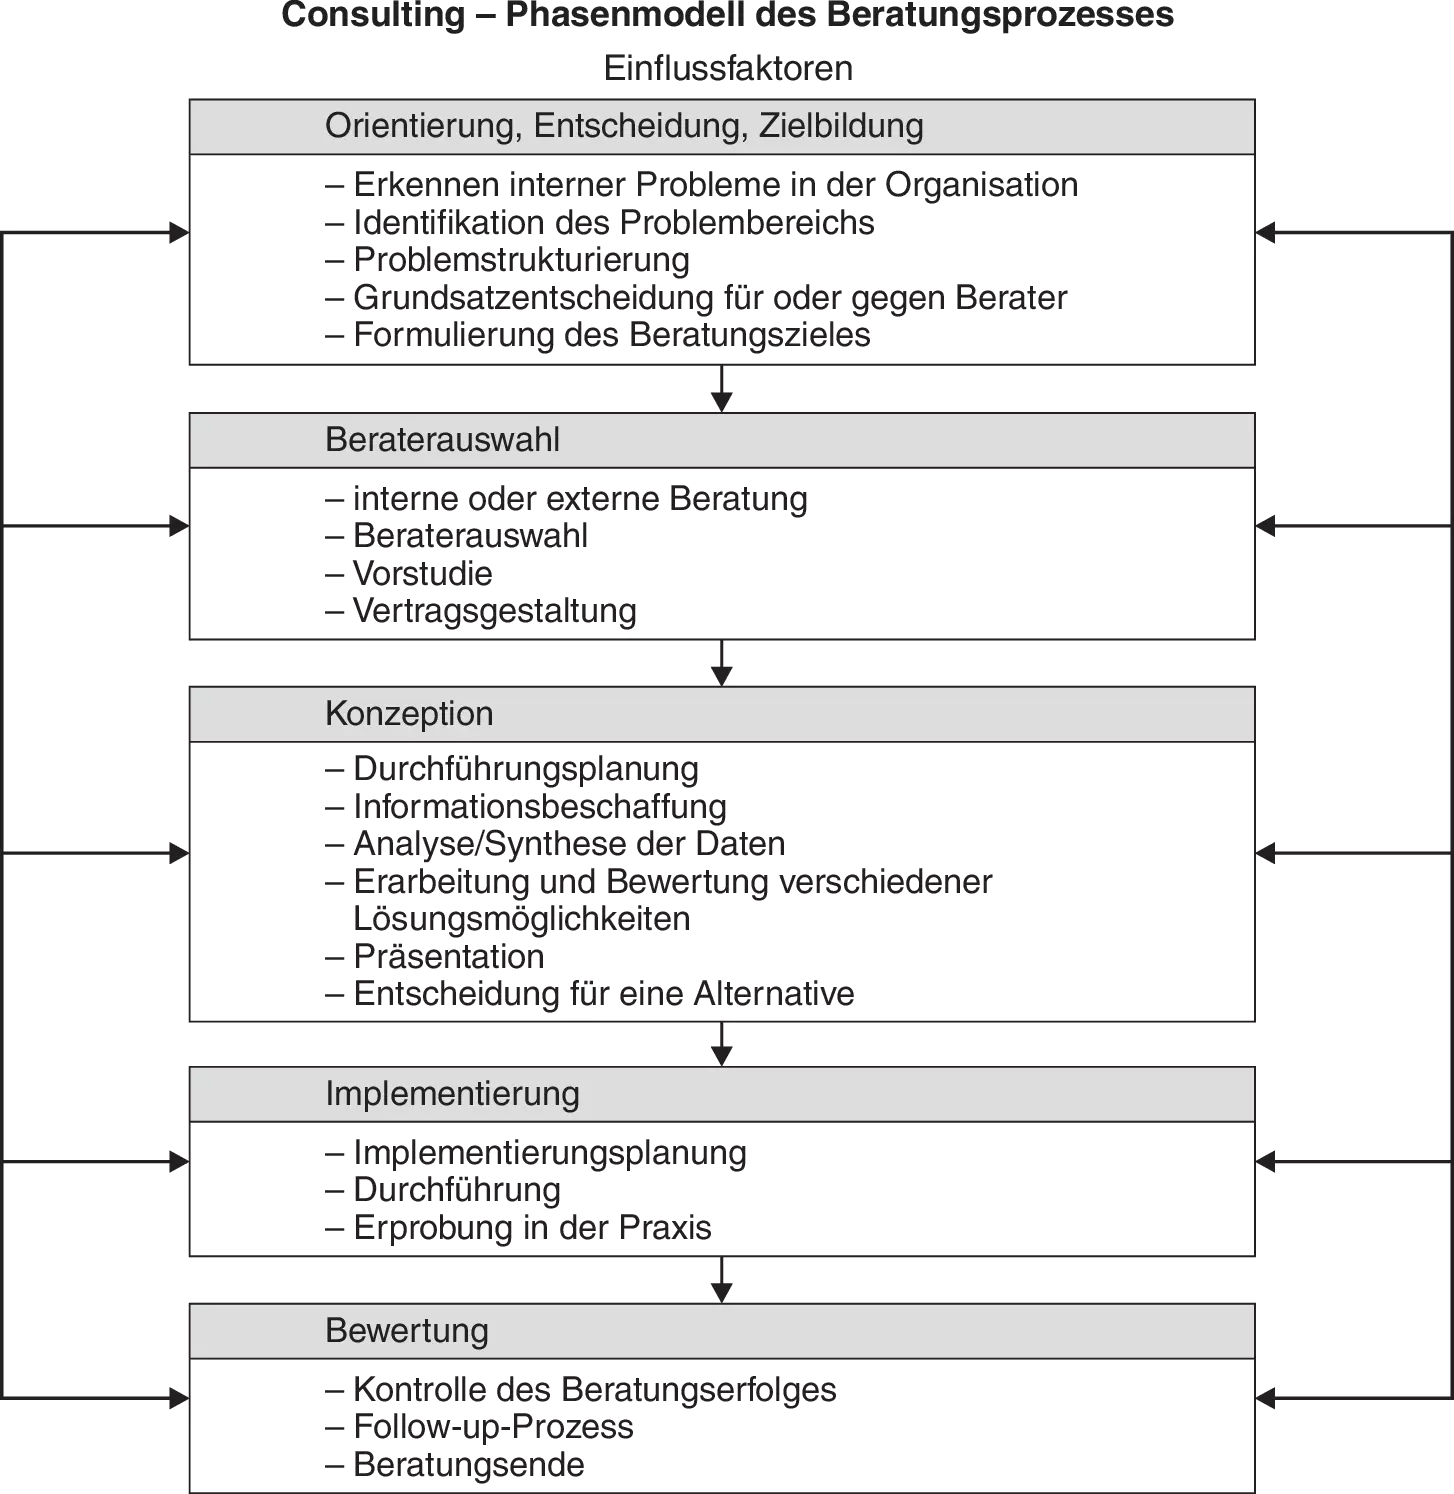
\includegraphics[scale=0.4]{./Bilder/Beratungsprozess.png}
    \caption[Phasenmodell eines Beratungsprozess]{Phasenmodell eines Beratungsprozess (\cite[Vgl.][]{gabler-beratung})}
\end{figure}
\\In der Praxis findet die Beratung in der Regel innerhalb von Projekten beim Kunden statt, die damit beginnen, dass der Kunde entweder auf das Beratungsunternehmen zukommt, oder eine Ausschreibung anfertigt, auf die sich das Beratungsunternehmen bewirbt. Danach erfolgt die Angebotserstellung durch das Beratungsunternehmen, in dem der Umfang des Projekts und die Leistungen der Berater festgehalten sind, sowie das Projektbudget. Die Abrechnung eines Projektes erfolgt entweder pauschal über einen Festpreis, oder über einen Stundensatz anhand der geleisteten Arbeitszeit. Sobald der Angebotszuschlag erhalten wurde, beginnt das Projekt mit der Konzeptionsphase, in der Informationen beschafft, Daten analysiert und verschiedene Lösungsmöglichkeiten in einem Fachkonzept erarbeitet werden. Sobald sich der Kunde für eine der Lösungen entschieden hat, beginnt mit der Implementierung die nächste Projektphase. In dieser findet die Durchführung der Lösung statt, sowie im Anschluss Tests und Fehlerbehebungen. Nach dem Abschluss der Implementierungsphase erfolgt die Abnahme, bzw. die Bewertung durch den Kunden, der auch eventuelle Nacharbeiten festsetzt oder nachfolgende Projekte in Aussicht stellt.\footcite[Vgl.][]{gabler-beratung}
\\Durch das nahende Supportende von SAP ERP (R/3) im Jahr xxxx (siehe Kapitel \ref{kap:R3}) stehen zur Zeit viele Unternehmen unter Zugzwang auf die neuste Generation S/4HANA zu aktualisieren. Dadurch ergeben sich für die Beratungsbranche viele Möglichkeiten Aufträge in Form von S/4HANA-Transformationsprojekten zu aquirieren. Auf der anderen Seite bietet der Druck auf die Unternehmen aber auch Chancen im selben Zug einschneidene Änderungen an den in SAP abgebildeten Geschäftsprozessen vorzunehemen, indem sich von Eigenentwicklungen und ineffizienten Prozessen getrennt wird und sie durch Prozesse des gängigen Industriestandard ersetzt.

\subsection{Vorgehensmodell S/4HANA Transformation}
\subsubsection{Aufbau}
Die adesso orange AG hat für die Durchführung von SAP S/4HANA Transformationen, mit Hilfe der im Unternehmen ansässigen Expertise, ein eigenes Vorgehensmodell entwickelt, dass auf vier durchzuführende Projektphasen basiert um eine vollumfängliche S/4HANA-Transformation durchzuführen. Dieses Vorgehensmodell wird unter dem Produktnamen \glqq{}adesso active Transformation\grqq{} vermarktet und kam bereits in einigen größeren Projekten zum Einsatz. 

\subsubsection{Phasen}

\subsubsection{Tools}

\subsubsection{Methodiken}

\subsubsection{Einordnung des BTT}